% An open arc of the circle S^1 (subspace of R^2), realized as the
% intersection of S^1 with an open disk (dotted).
% Source: book/tex/topology/top-more.tex (§ Subspaces).
\documentclass[border=2mm]{standalone}
\usepackage{amssymb}
\usepackage{tikz}
\begin{document}
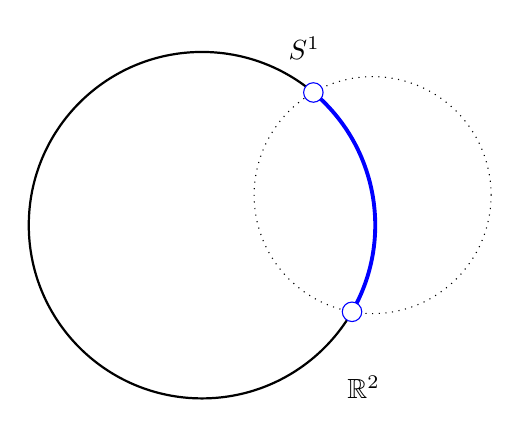
\begin{tikzpicture}[scale=2.2]
  \draw[black, line width=0.8pt] (0,0) circle (1);
  \node at (60:1.18) {$S^1$};
  \node at (-45:1.32) {$\mathbb{R}^2$};
  % open disk centered at dir(10) passing through A=dir(-30): radius 2 sin(20 deg)
  \draw[dotted] (10:1) circle (0.6840);
  \draw[blue, line width=1.4pt] (-30:1) arc (-30:50:1);
  \draw[blue, fill=white] (-30:1) circle (1.6pt);
  \draw[blue, fill=white] (50:1) circle (1.6pt);
\end{tikzpicture}
\end{document}
